\appendix
\chapter{Appendix}
\section{Cross Correlations}
\begin{figure}[h]
	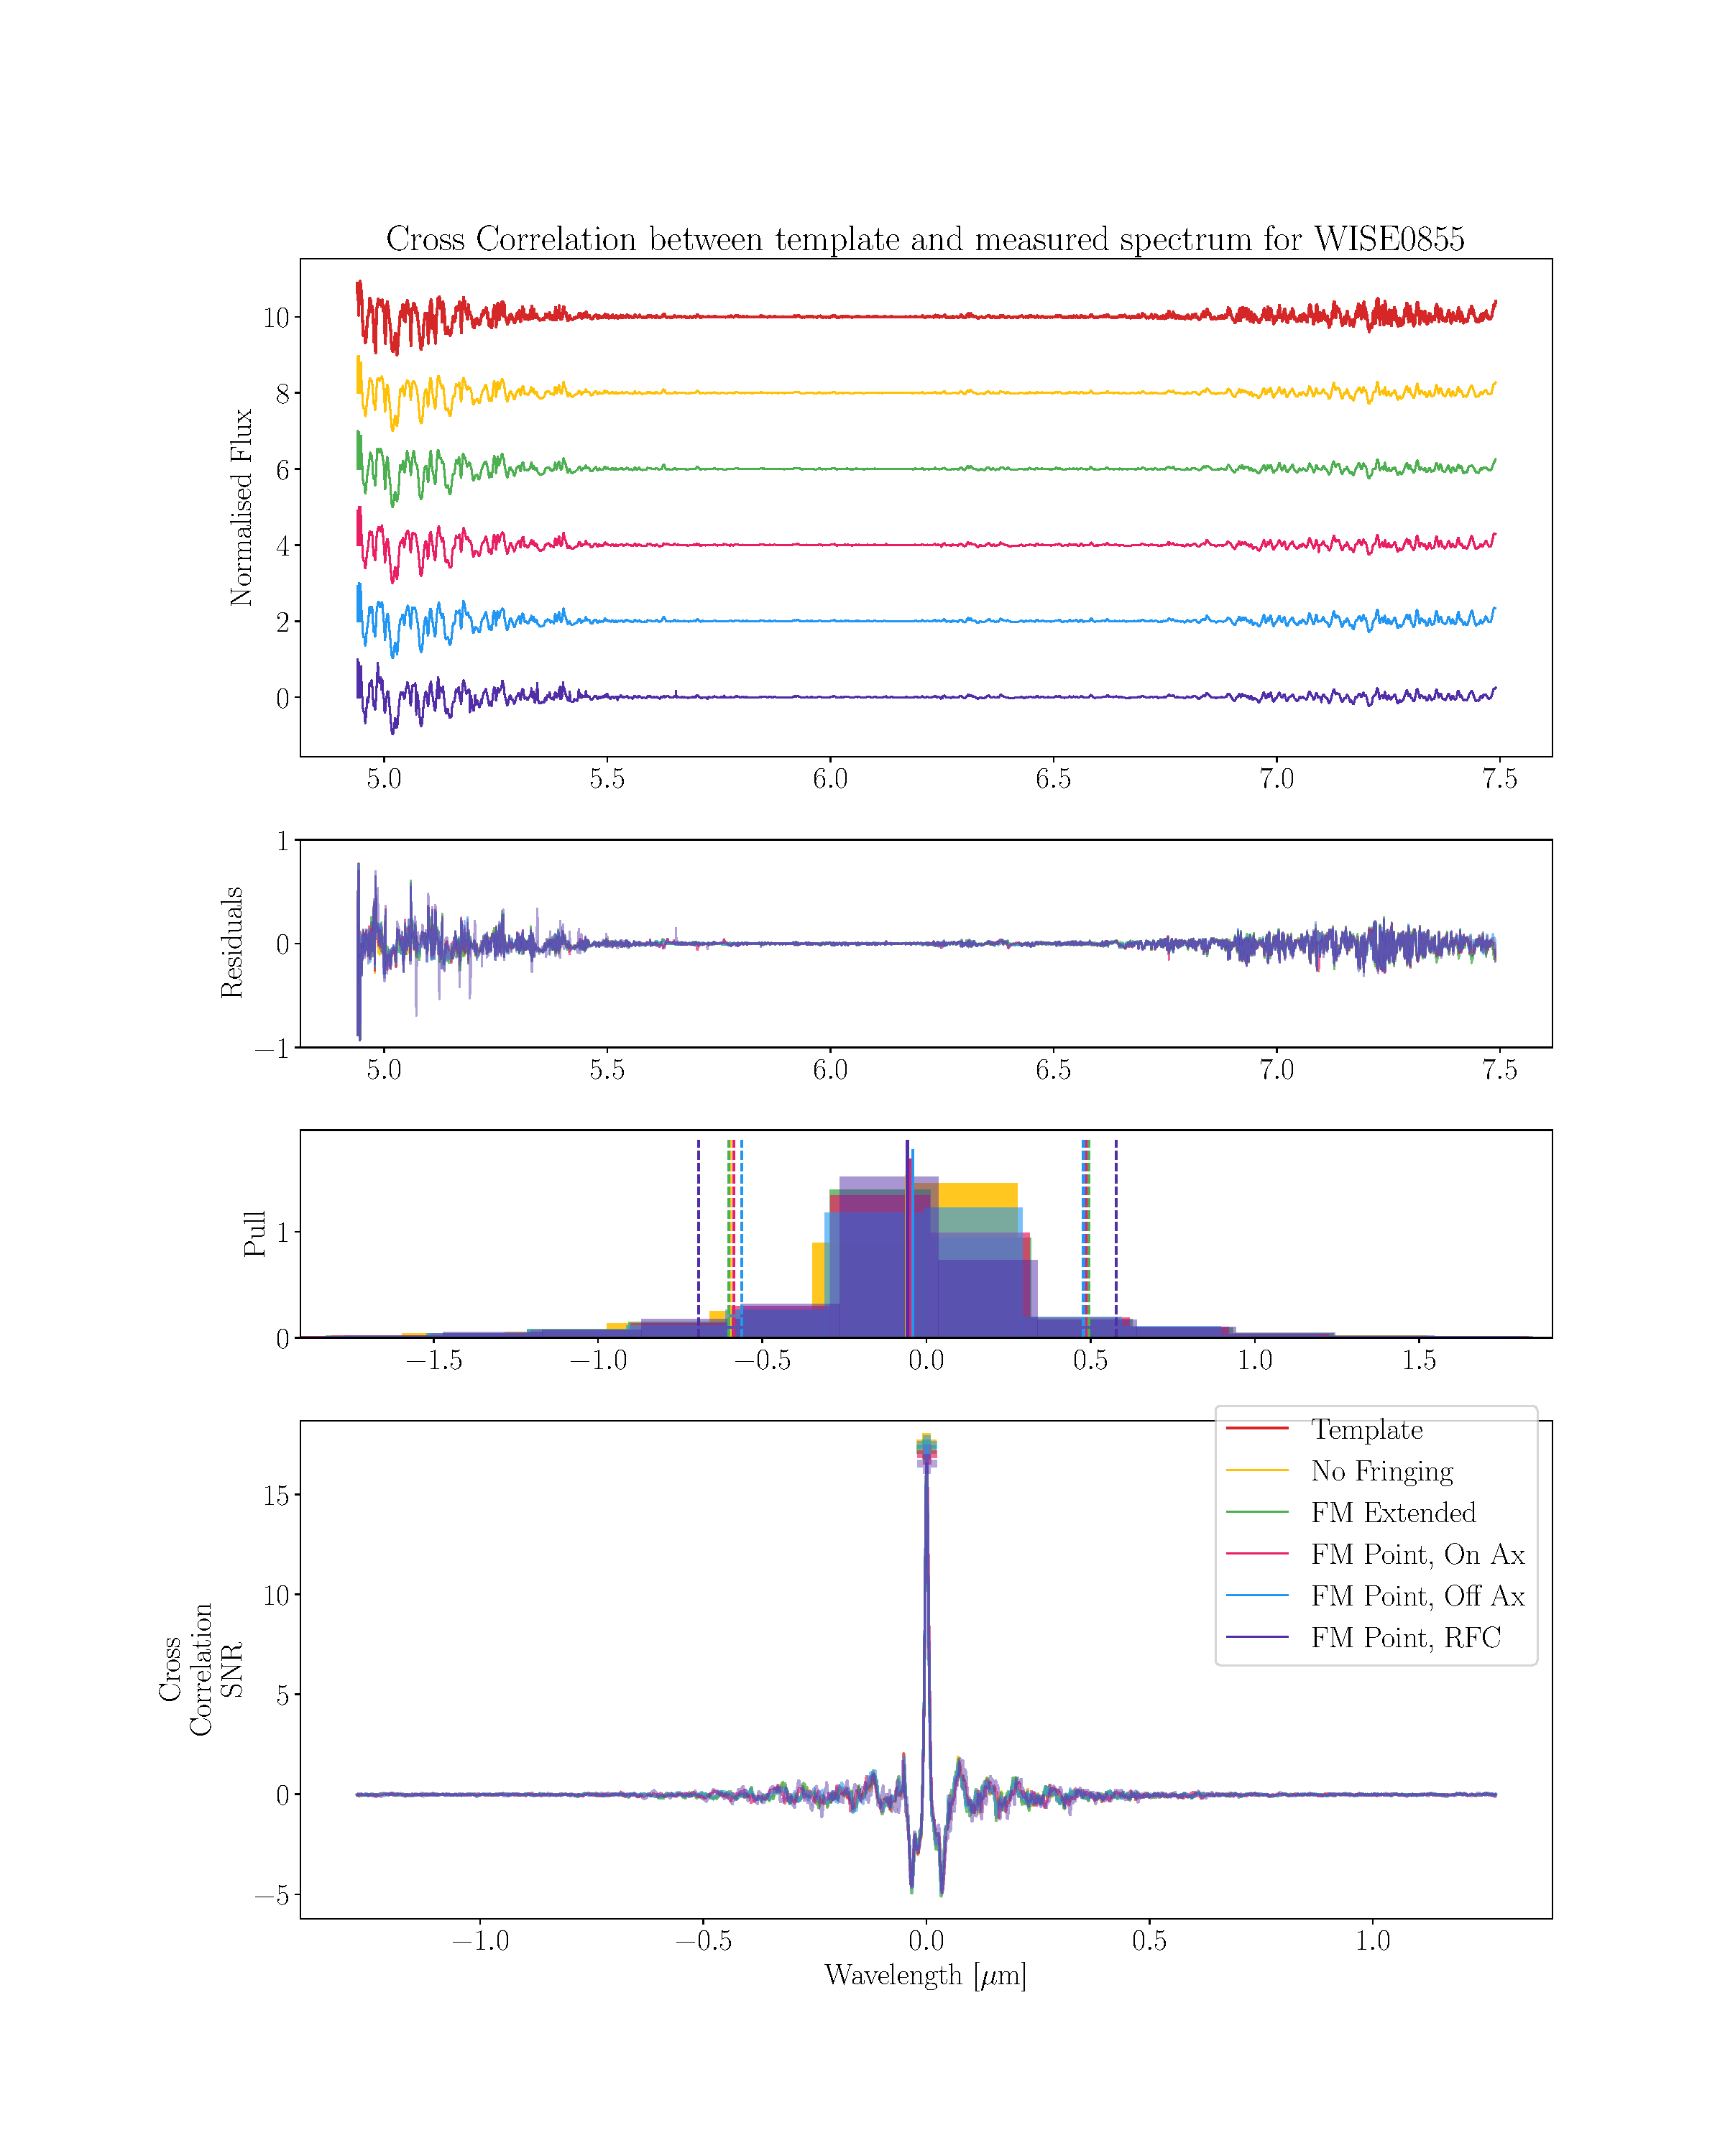
\includegraphics[width=\linewidth,trim=4cm 3.5cm 4cm 4.5cm, clip]{WISECrossCorTemplate}
	\caption{Cross correlation between the input template and the extracted spectra for WISE0855.}
\end{figure}
\begin{figure}[h]
	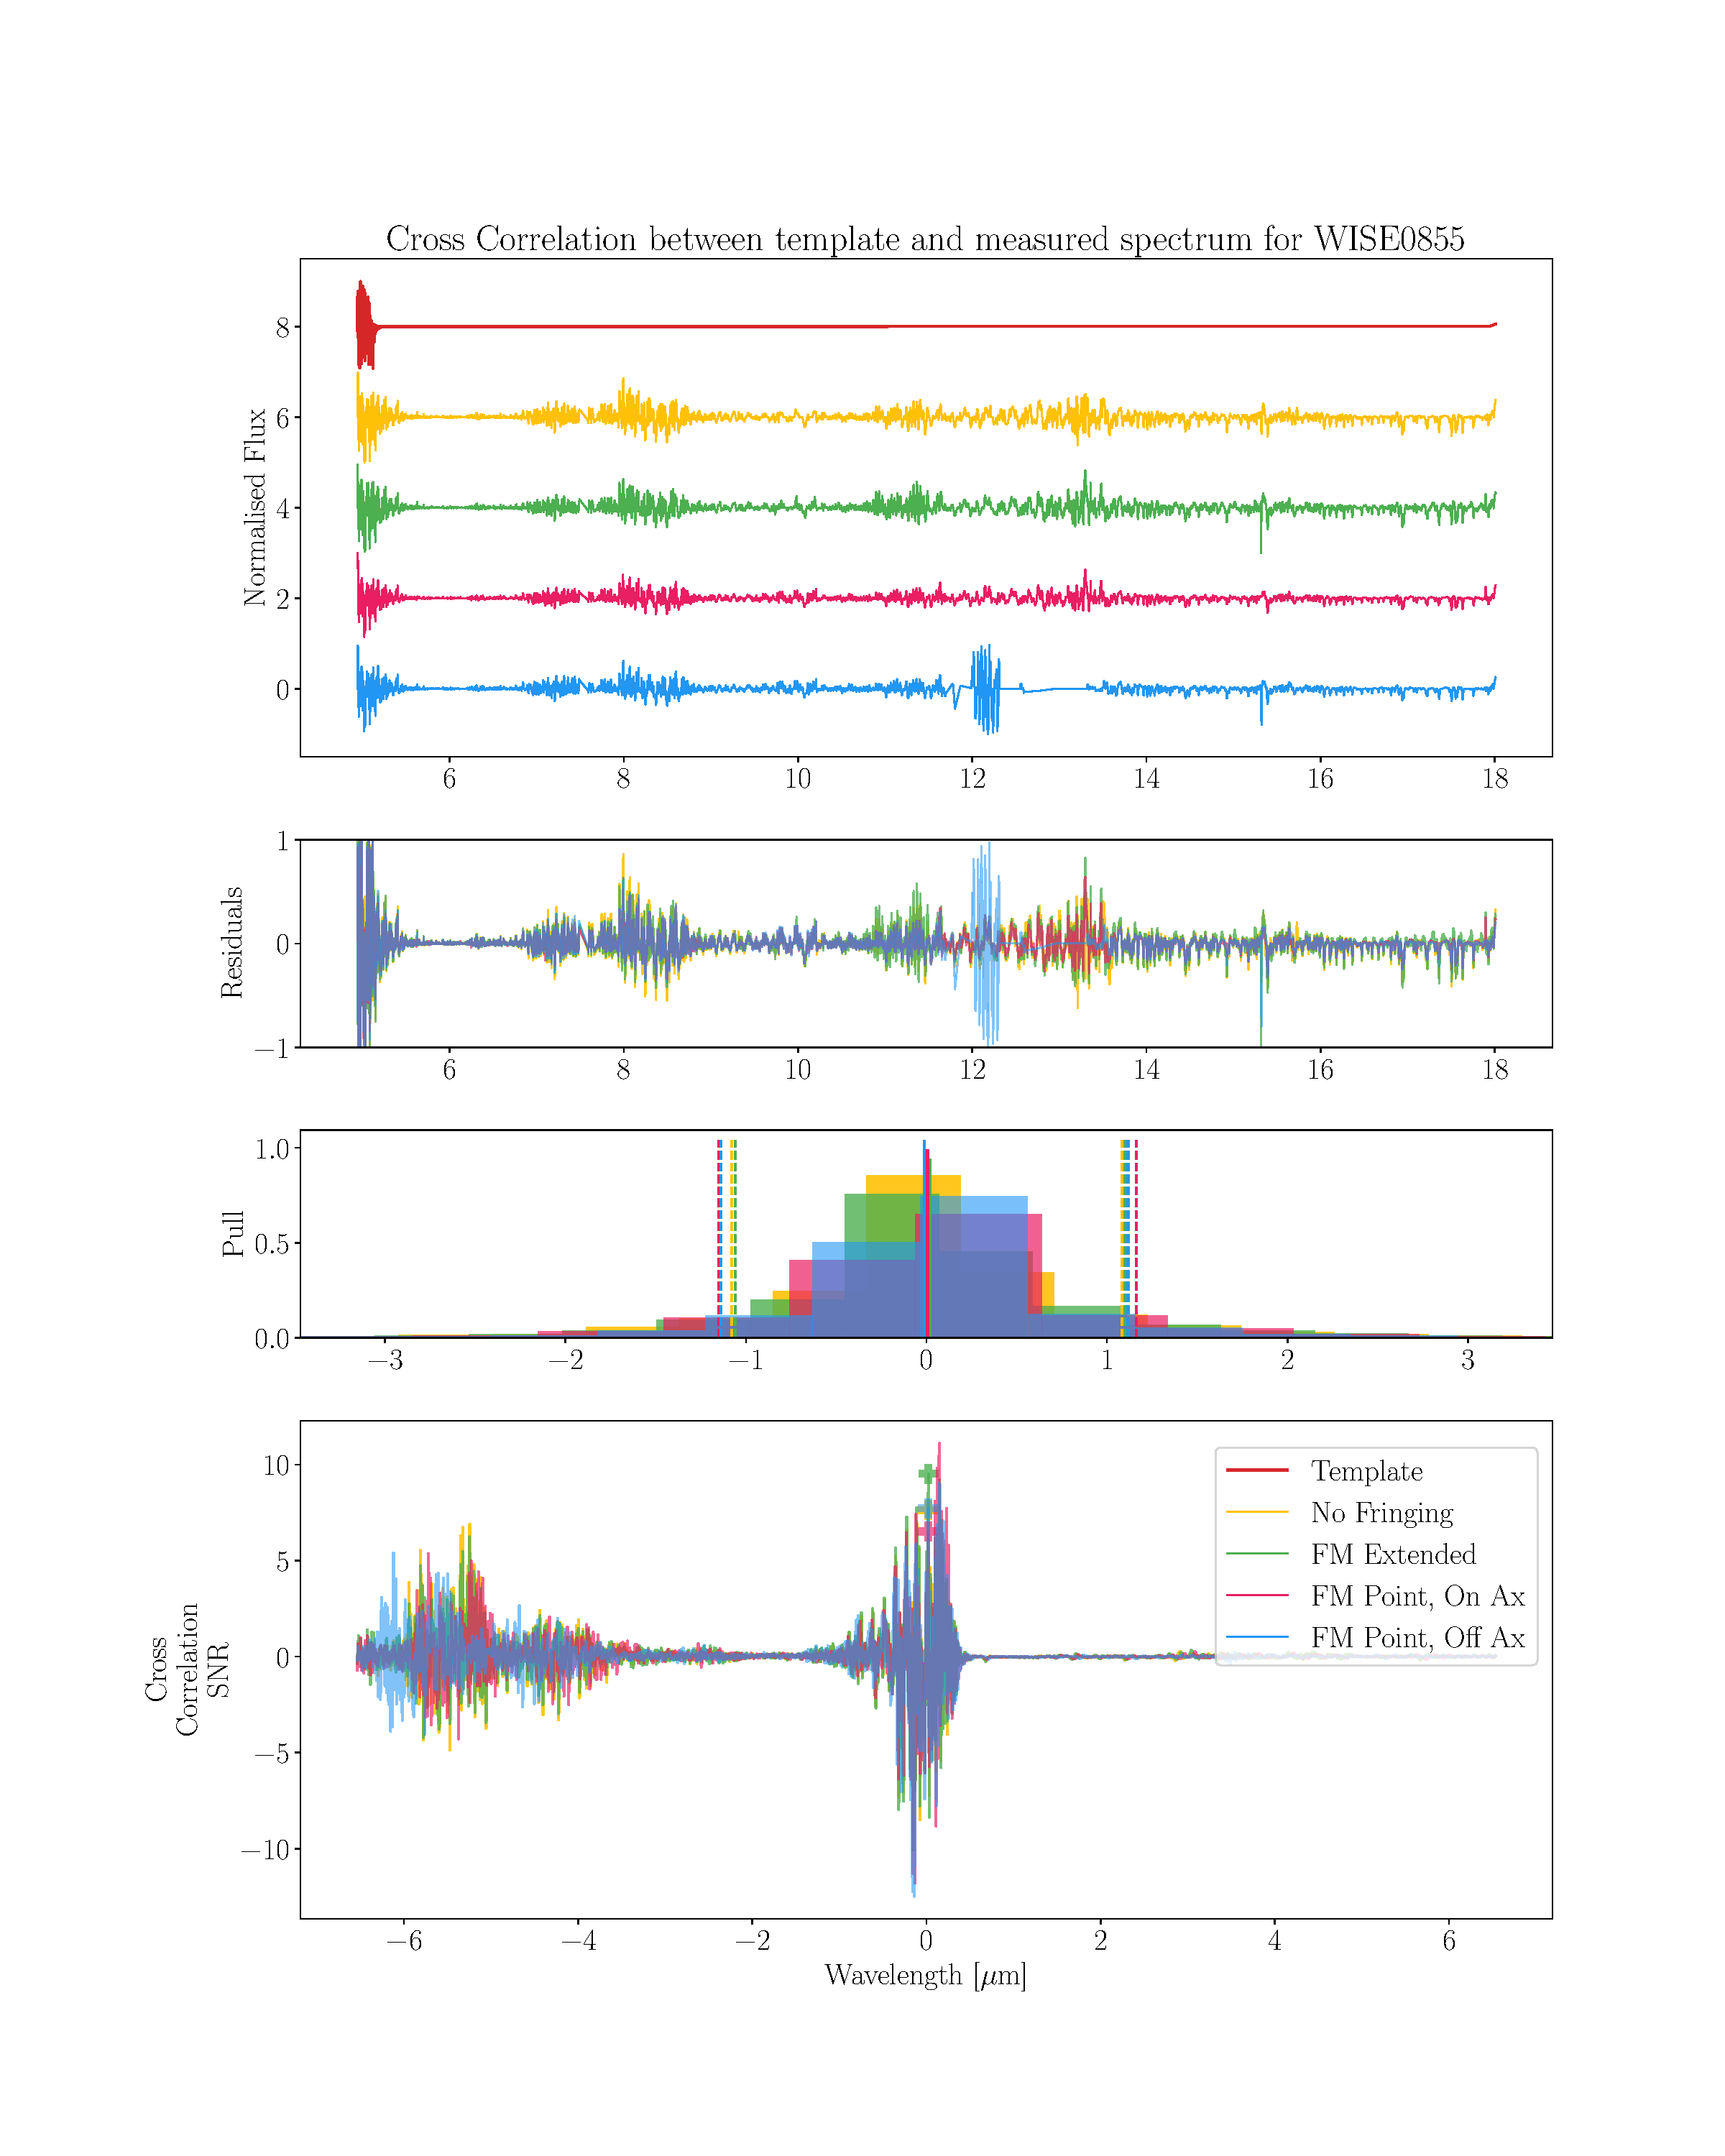
\includegraphics[width=\linewidth,trim=4cm 3.5cm 4cm 4.5cm, clip]{WISECO}
	\caption{Single species cross correlation between CO and WISE0855. The lack of significant spectral coverage results in a false positive detection.}
	\label{fig:wiseco}
\end{figure}
\begin{figure}[h]
	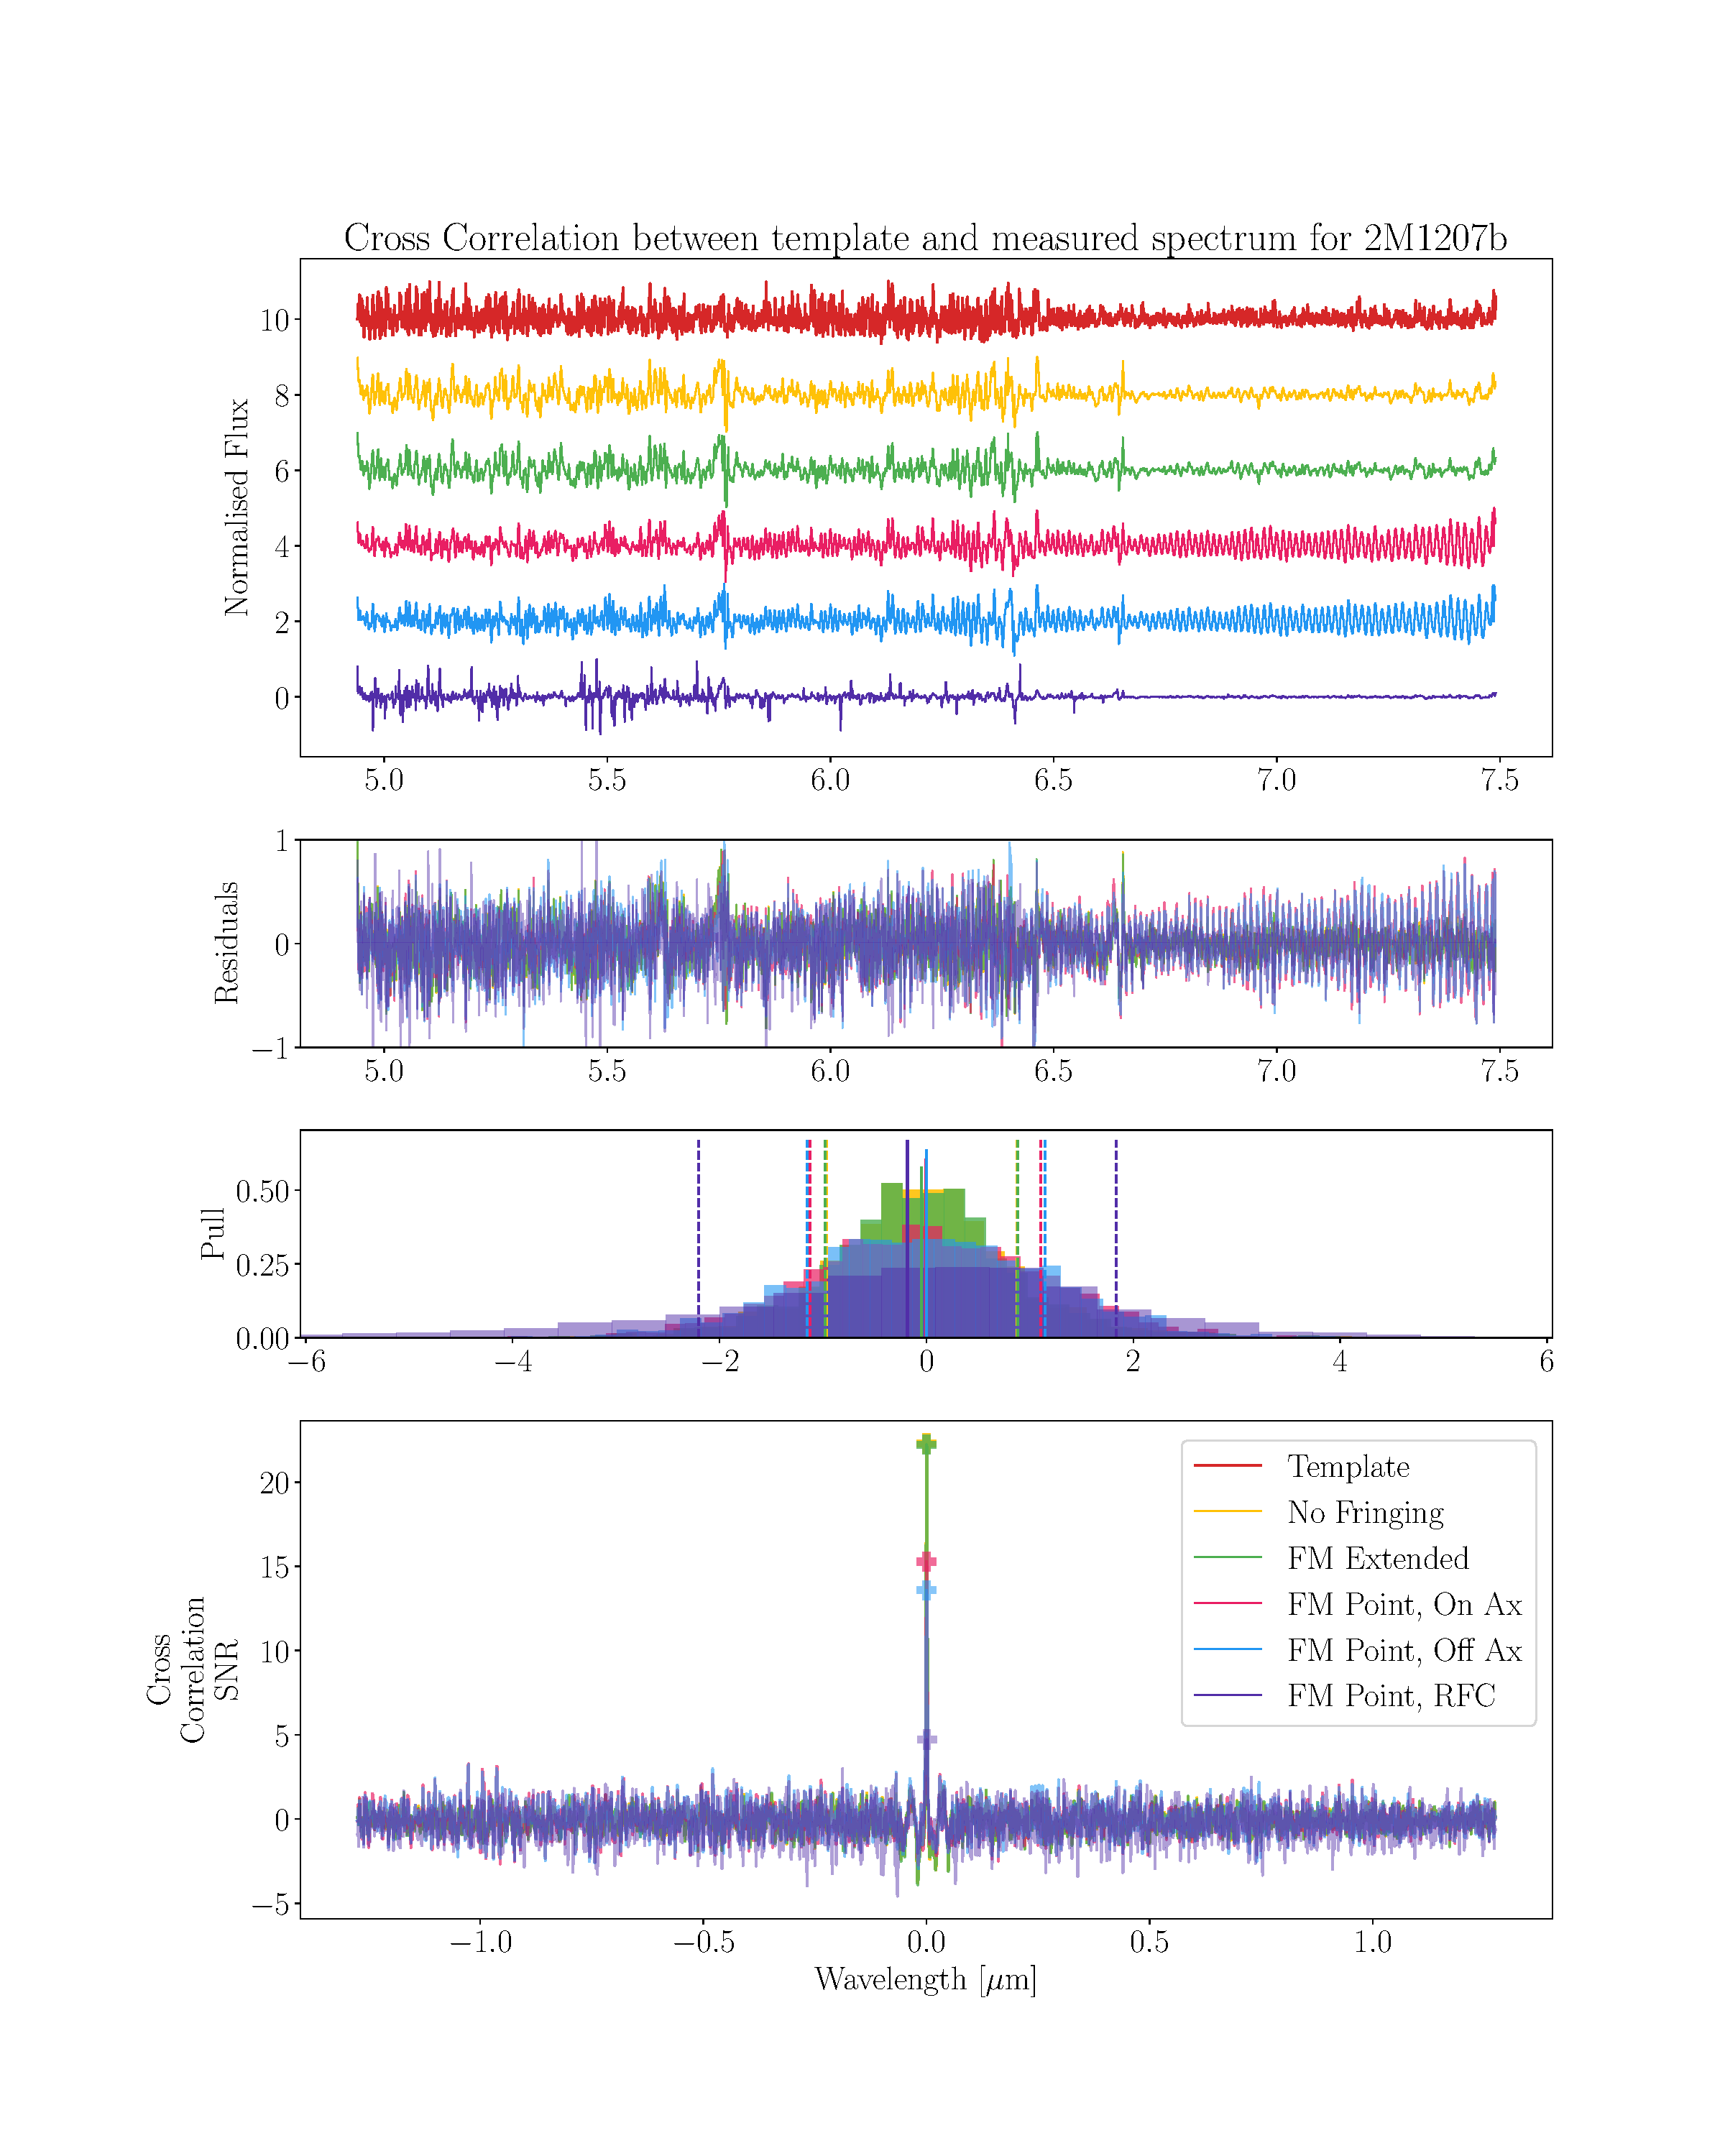
\includegraphics[width=\linewidth,trim=4cm 3.5cm 4cm 4.5cm, clip]{2M1207bCrossCorTemplate}
	\caption{Cross correlation between the input template and the extracted spectra for 2M1207b.}
\end{figure}
\begin{figure}[h]
	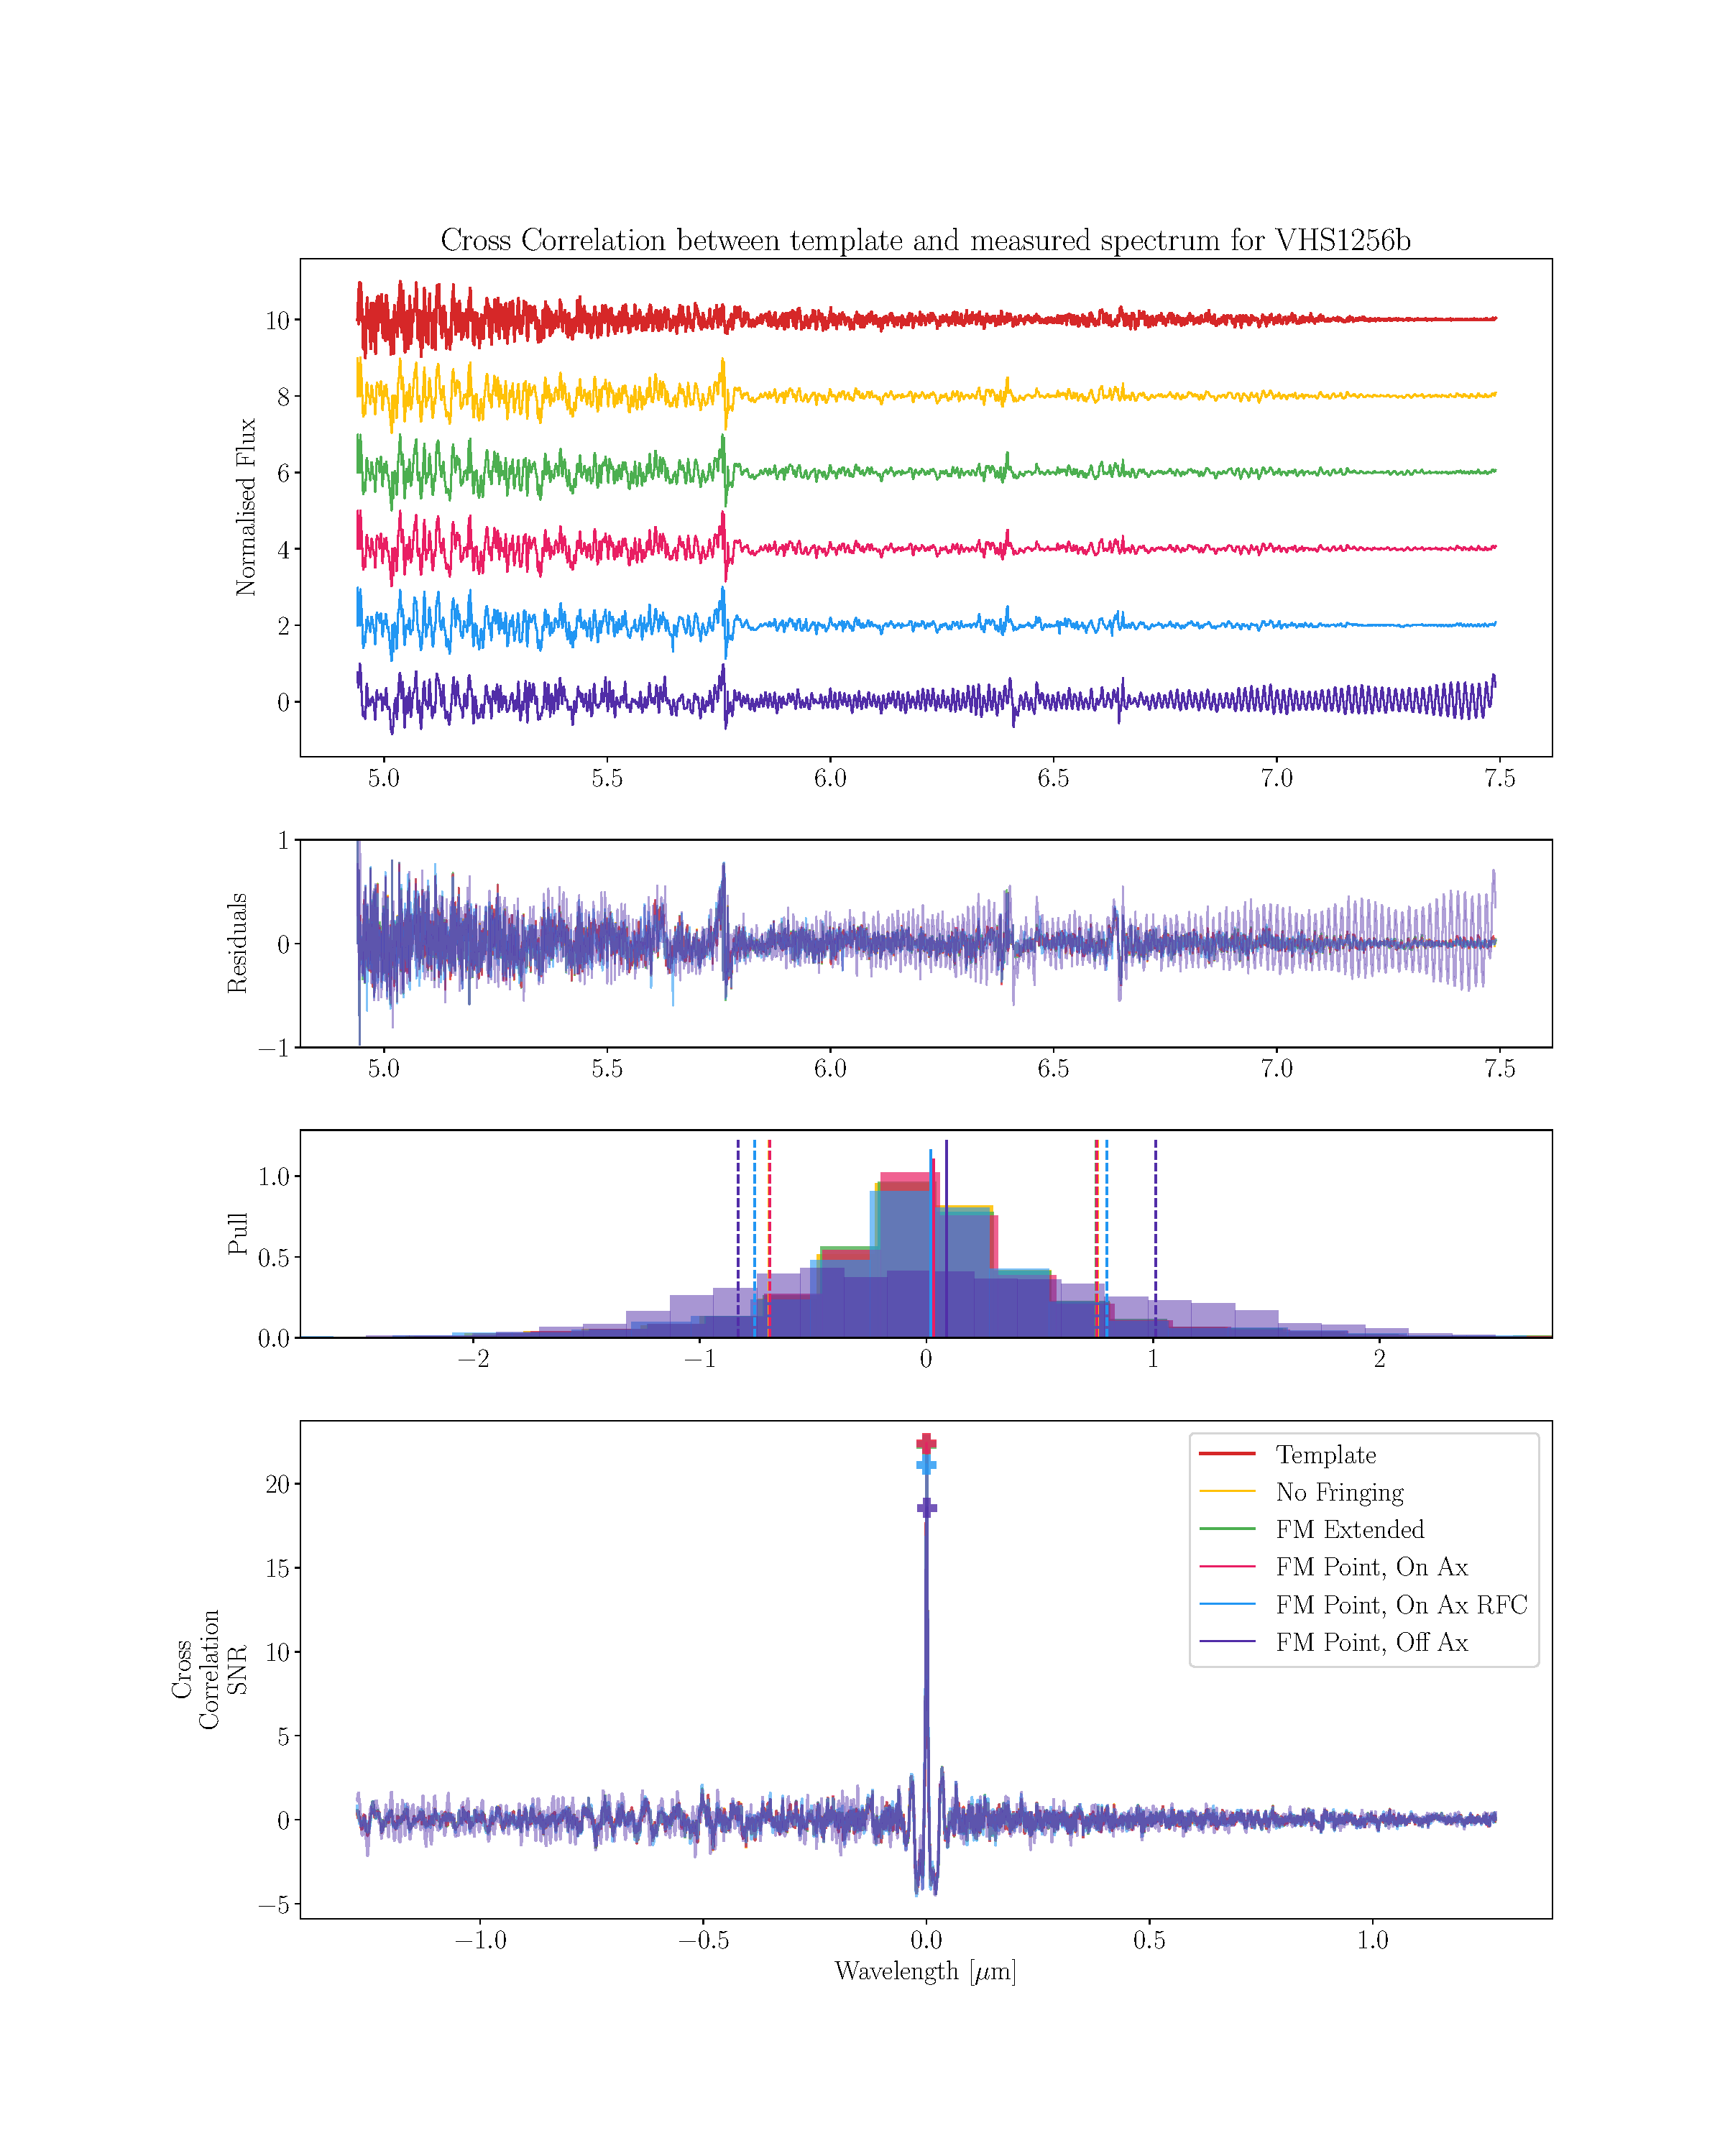
\includegraphics[width=\linewidth,trim=4cm 3.5cm 4cm 4.5cm, clip]{VHSCrossCorTemplateUncorrOnAxCH1}
	\caption{Cross correlation between the input template and the extracted spectra for VHS1256b. In this plot, the on axis point source has not been corrected with the extended source fringe flat, resulting in a higher SNR than with the correction.}
\end{figure}

\clearpage
\section{Package Requirements}
\verbatiminput{Chapters/requirements.txt}
